\documentclass[a4paper]{article}
\usepackage[utf8]{inputenc}
\usepackage{amssymb}
\usepackage{hyperref}
\usepackage{enumitem}
\usepackage{listings}
\usepackage{esvect}
\usepackage{float}
\usepackage{graphicx}
\usepackage{xcolor}
\usepackage{todonotes}
\usepackage{pgfplots}
\usepackage{verbatim}
\usepackage{siunitx}
\pgfplotsset{compat=1.10}
\usepgfplotslibrary{fillbetween}
\usetikzlibrary{patterns}
\usepackage{mathtools}
\usepackage{centernot}
\usepackage{subcaption}

\usepackage{listings}
\usepackage{color} %red, green, blue, yellow, cyan, magenta, black, white
\definecolor{mygreen}{RGB}{28,172,0} % color values Red, Green, Blue
\definecolor{mylilas}{RGB}{170,55,241}

\lstset{language=Matlab,%
    %basicstyle=\color{red},
    breaklines=true,%
    morekeywords={matlab2tikz},
    keywordstyle=\color{blue},%
    morekeywords=[2]{1}, keywordstyle=[2]{\color{black}},
    identifierstyle=\color{black},%
    stringstyle=\color{mylilas},
    commentstyle=\color{mygreen},%
    showstringspaces=false,%without this there will be a symbol in the places where there is a space
    numbers=left,%
    numberstyle={\tiny \color{black}},% size of the numbers
    numbersep=9pt, % this defines how far the numbers are from the text
    emph=[1]{for,end,break},emphstyle=[1]\color{red}, %some words to emphasise
    %emph=[2]{word1,word2}, emphstyle=[2]{style},    
}


\title{Computer Vison Exercise 3}
\author{Marco Deuscher(977776) & Carolin Schindler(978616)}
\date{May 2019}

\begin{document}

\maketitle
\section{Histogram equalization}
In this exercise histogram equalization is used. It is a method to improve the distribution of intensity values in an image.\\
First the image is loaded using Matlabs build in \textit{imread}-function. Then the function developed in Sheet 1 is used to create a histogram. The created Histogram and the original image can be seen in fig. \ref{plot01}.\\
A cumulative histogram was then implemented using the following formula
\begin{equation*}
    s_k = \sum_{j=0}^kp(g_j)\quad \text{where $p(g_j)$ is the probability of a specific grey scale}
\end{equation*}
The cumulative histogram can be seen in fig. \ref{plot01}.\\
Then each intensity k in the original image was mapped onto the closest value of $s_k * 255$.\\
The improved image can be seen in fig. \ref{plot01}.

\begin{figure}[htp]
    \centering
    \lstinputlisting{sh03ex01.m}
    \caption{Matlab code for exercise 1}
    \label{ex01}
\end{figure}

\begin{figure}[htp]
    \centering
    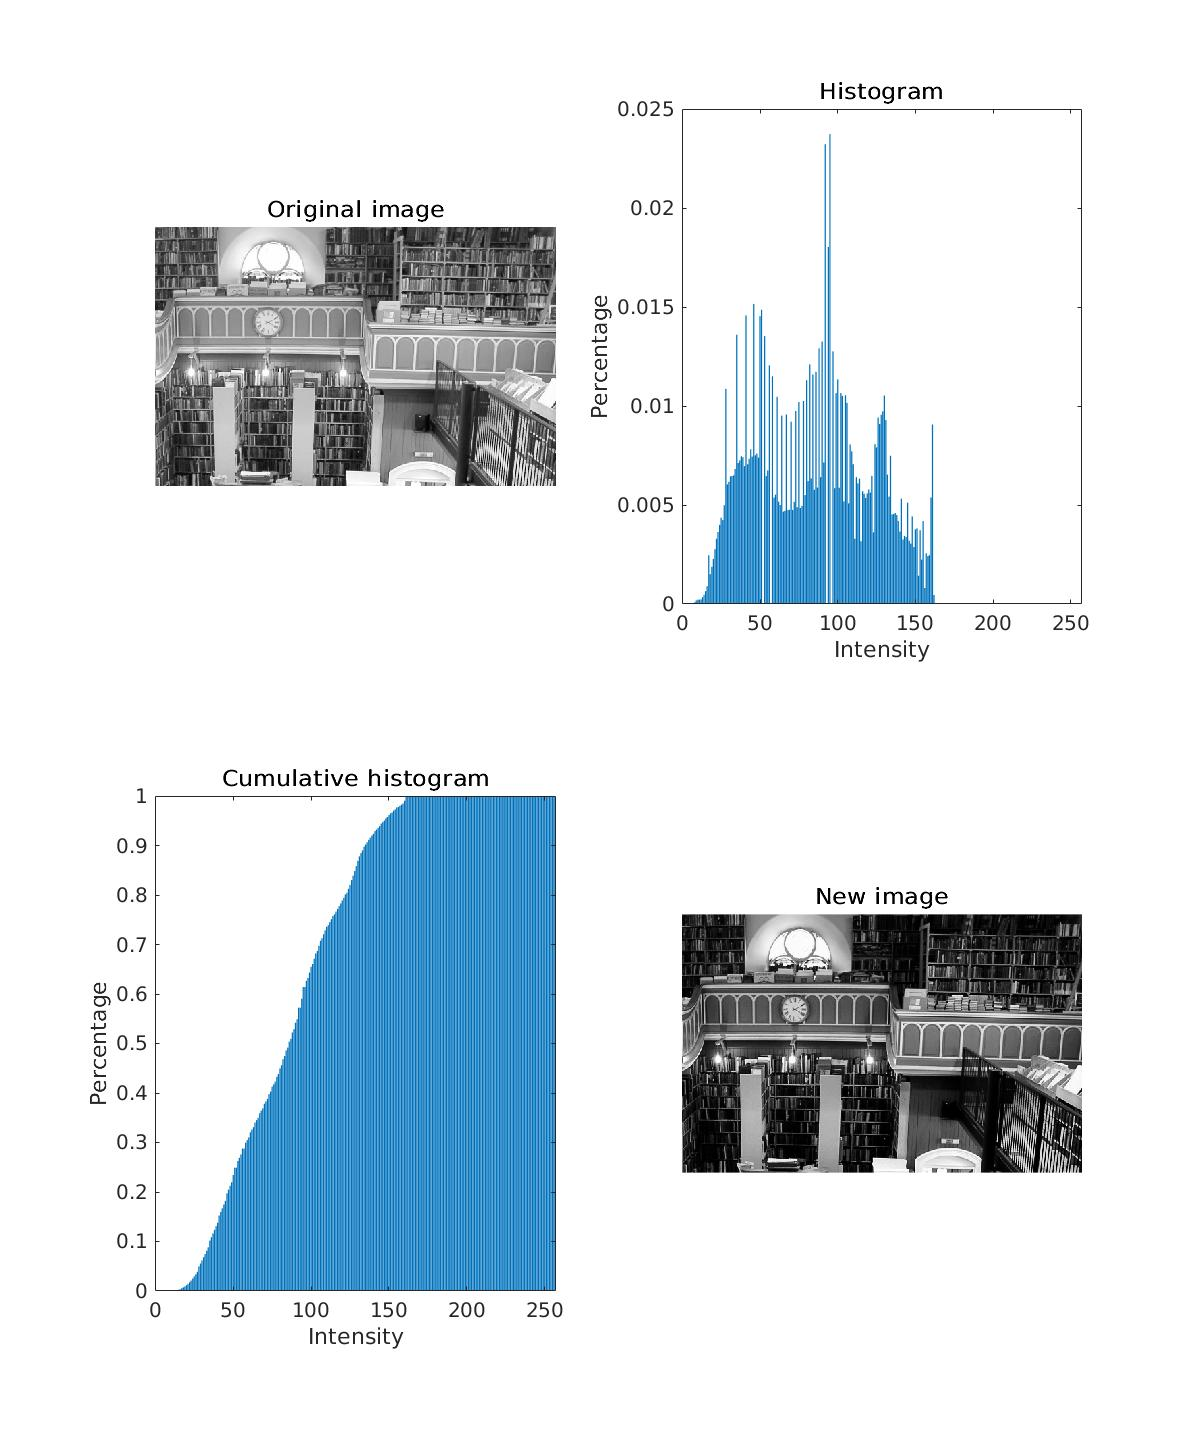
\includegraphics[width=\textwidth]{plot01.jpg}
    \caption{Plots for exercise 1}
    \label{plot01}
\end{figure}

\newpage

\section{Image gradients}
The formula for the convolution is 
\begin{equation*}
    \sum_k\sum_j I[x-k,y-j]G[k,j]
\end{equation*}
\paragraph{(1)}
The effect of the sign in the Sobel-Operator is that it defines the reading direction. If the intensity decreases from left to right $I_{x,y}<0$.\\
If the intensity increases form left to right $I_{x,y}>0$.\\
Inverting the sign flips the above stated correlations.\\
Analogous for the y-Axis.

\paragraph{(2)}
\paragraph{(II)}
\begin{align*}
    I_x &= \begin{bmatrix}
        0 & 0 & 0\\
        0 & 0 & 255\\
        0 & 0 & 255\\
        \end{bmatrix}
         * 
         \begin{bmatrix}
        1 & 0 & -1\\
        2 & 0 & -2\\
        1 & 0 & -1\\
        \end{bmatrix}
        = 2*255+255 = 765\\
        I_y &= \begin{bmatrix}
        0 & 0 & 0\\
        0 & 0 & 255\\
        0 & 0 & 255\\
        \end{bmatrix}
         * 
         \begin{bmatrix}
        -1 & -2 & -1\\
        0 & 0 & -0\\
        1 & 2 & -1\\
        \end{bmatrix}
        = -255\\
        \nabla I &= (I_x,I_y)^T = (765,-255)^T\\
        \| \nabla I\| &= \sqrt{765^2+(-255)^2} = 806,38\\
        \Theta_I &= \operatorname{arctan}(\frac{I_y}{I_x}) = -0.32
\end{align*}

\paragraph{(III)}
\begin{align*}
    I_x &= \begin{bmatrix}
        255 & 255 & 255\\
        255 & 255 & 255\\
        255 & 255 & 0\\
        \end{bmatrix}
         * 
         \begin{bmatrix}
        1 & 0 & -1\\
        2 & 0 & -2\\
        1 & 0 & -1\\
        \end{bmatrix}
        = -255\\
        I_y &= \begin{bmatrix}
        255 & 255 & 255\\
        255 & 255 & 255\\
        255 & 255 & 0\\
        \end{bmatrix}
         * 
         \begin{bmatrix}
        -1 & -2 & -1\\
        0 & 0 & -0\\
        1 & 2 & -1\\
        \end{bmatrix}
        = 255\\
        \nabla I &= (I_x,I_y)^T = (-255,255)^T\\
        \| \nabla I\| &= \sqrt{765^2+(-255)^2} = 360,62\\
        \Theta_I &= \operatorname{arctan}(\frac{I_y}{I_x}) = \frac{3}{4}\pi
\end{align*}

\paragraph{(IV)}
\begin{align*}
    I_x &= \begin{bmatrix}
        255 & 255 & 255\\
        255 & 255 & 255\\
        255 & 0 & 0\\
        \end{bmatrix}
         * 
         \begin{bmatrix}
        1 & 0 & -1\\
        2 & 0 & -2\\
        1 & 0 & -1\\
        \end{bmatrix}
        = -255\\
        I_y &= \begin{bmatrix}
        255 & 255 & 255\\
        255 & 255 & 255\\
        255 & 0 & 0\\
        \end{bmatrix}
         * 
         \begin{bmatrix}
        -1 & -2 & -1\\
        0 & 0 & -0\\
        1 & 2 & -1\\
        \end{bmatrix}
        = 765\\
        \nabla I &= (I_x,I_y)^T = (-255,765)^T\\
        \| \nabla I\| &= \sqrt{765^2+(-255)^2} = 806,38\\
        \Theta_I &= \operatorname{arctan}(\frac{I_y}{I_x}) = -1,24
\end{align*}

\paragraph{(V)}
\begin{align*}
    I_x &= \begin{bmatrix}
        255 & 0 & 0\\
        255 & 0 & 0\\
        255 & 0 & 0\\
        \end{bmatrix}
         * 
         \begin{bmatrix}
        1 & 0 & -1\\
        2 & 0 & -2\\
        1 & 0 & -1\\
        \end{bmatrix}
        = -1020\\
        I_y &= \begin{bmatrix}
        255 & 0 & 0\\
        255 & 0 & 0\\
        255 & 0 & 0\\
        \end{bmatrix}
         * 
         \begin{bmatrix}
        -1 & -2 & -1\\
        0 & 0 & -0\\
        1 & 2 & -1\\
        \end{bmatrix}
        = 0\\
        \nabla I &= (I_x,I_y)^T = (-1020,0)^T\\
        \| \nabla I\| &= \sqrt{765^2+(-255)^2} = 1020\\
        \Theta_I &= \operatorname{arctan}(\frac{I_y}{I_x}) = 0\\
\end{align*}

\paragraph{(VI)}
\begin{align*}
    I_x &= \begin{bmatrix}
        0 & 255 & 255\\
        0 & 255 & 255\\
        0 & 0 & 0\\
        \end{bmatrix}
         * 
         \begin{bmatrix}
        1 & 0 & -1\\
        2 & 0 & -2\\
        1 & 0 & -1\\
        \end{bmatrix}
        = 765\\
        I_y &= \begin{bmatrix}
        0 & 255 & 255\\
        0 & 255 & 255\\
        0 & 0 & 0\\
        \end{bmatrix}
         * 
         \begin{bmatrix}
        -1 & -2 & -1\\
        0 & 0 & -0\\
        1 & 2 & -1\\
        \end{bmatrix}
        = 765\\
        \nabla I &= (I_x,I_y)^T = (765,765)^T\\
        \| \nabla I\| &= \sqrt{765^2+(-255)^2} = 1081,87\\
        \Theta_I &= \operatorname{arctan}(\frac{I_y}{I_x}) = \operatorname{arctan}(1)\\
\end{align*}

\paragraph{(3)}
In the following Matlab exercise the given image \textit{circles.png} is read in using \textit{imread}. The image is then normalized and the filters $I_x$ and $I_y$ are applied. Then for each pixel the magnitude of the gradient and the orientation of the gradient was computed. The results can be seen in fig. \ref{plot02}. The Matlab code which was used to create the plots can be seen in fig. \ref{ex02}.


\begin{figure}[htp]
    \centering
    \lstinputlisting{sh03ex02.m}
    \caption{Matlab code for exercise 2}
    \label{ex02}
\end{figure}

\begin{figure}[htp]
    \centering
    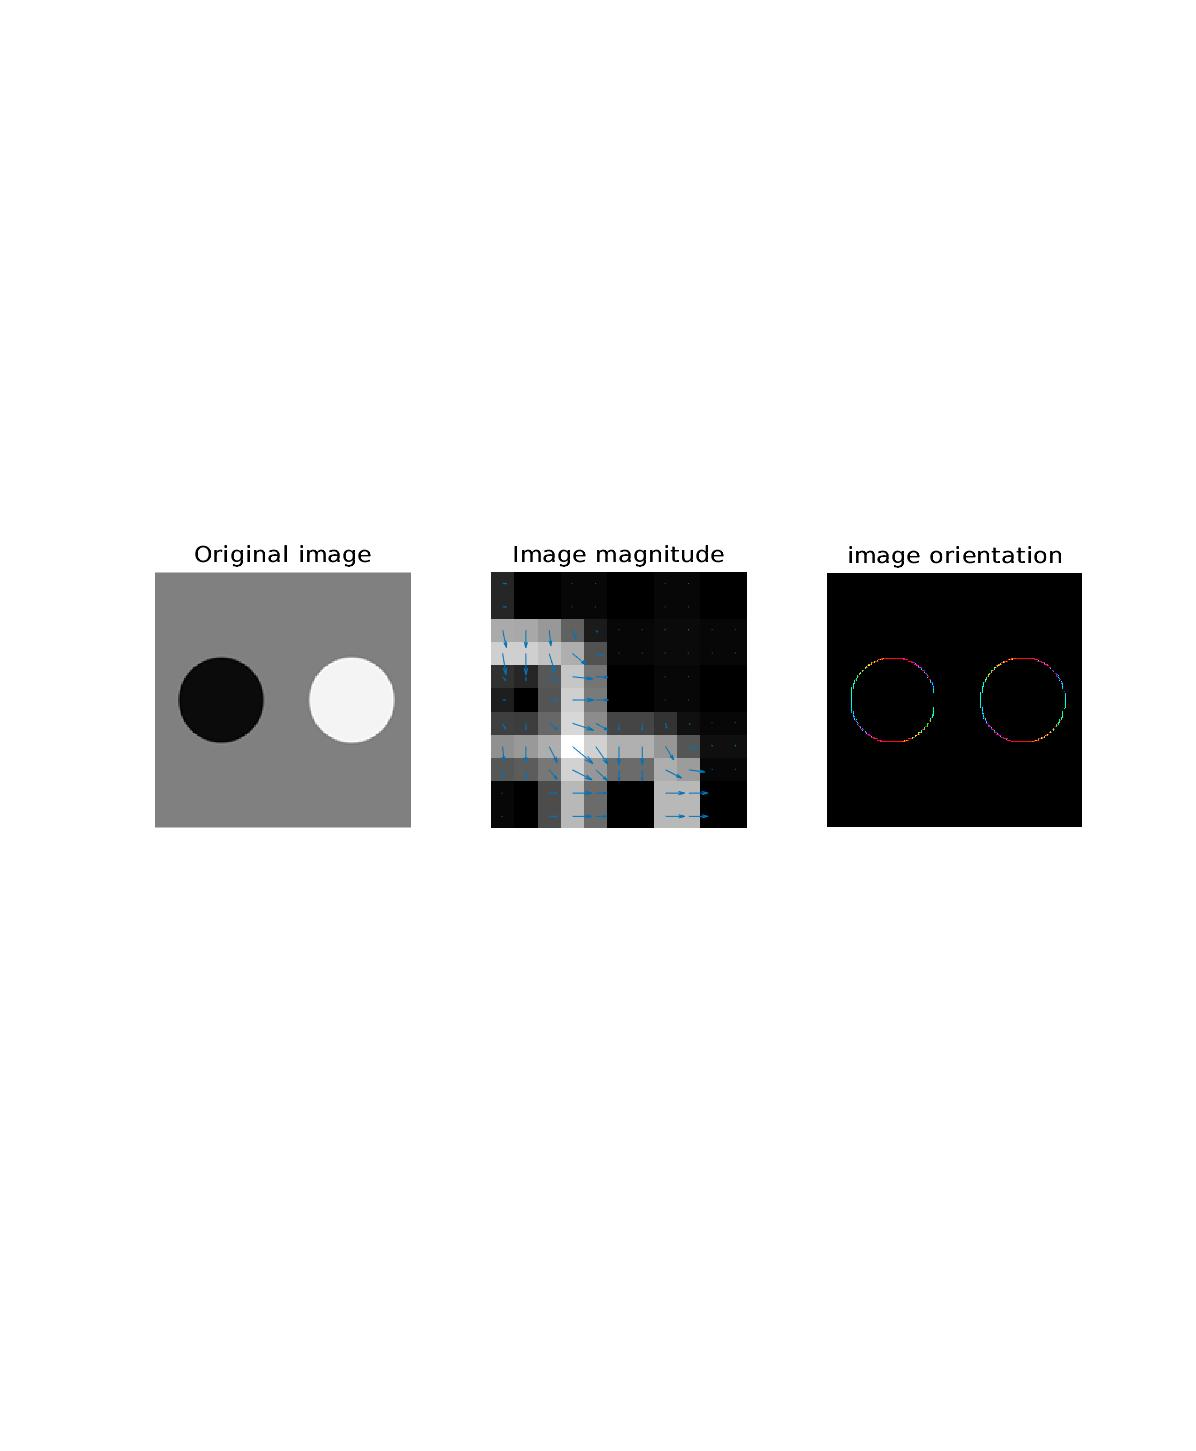
\includegraphics[width=\textwidth]{plot02.jpg}
    \caption{Plots for exercise 2}
    \label{plot02}
\end{figure}

\newpage
\section{Deconvolution}
The goal of this exercise is to remove the effect of a known filter.\\
First the filters are being loaded and displayed. They can been seen in the frequency domain, as well as in the spatial domain in fig. \ref{plot03}.\\
The filters are plotted logarithmically in the frequency domain to ensure that more values are visible.\\
The convolution in the frequency domain is applied by multiplying two signals. So the inverse operation is a divison.\\
The result of the deconvolution can be senn in fig. \ref{plot03}.

\paragraph{(3)}
The second filter cancels out higher frequencies. By deconvolving the filtered image these higher frequencies get amplified and can be seen in the second image as horizontal lines.

\paragraph{(4)}
The filter in the frequency domain contains zeros. As the filter is applied to the image by multiplying it with the image, those frequencies cancel out and cannot be reconstructed. Thus a perfect restoration of the image is not possible.


\begin{figure}[htp]
    \centering
    \lstinputlisting{sh03ex03.m}
    \caption{Matlab code for exercise 3}
    \label{ex03}
\end{figure}

\begin{figure}[htp]
    \centering
    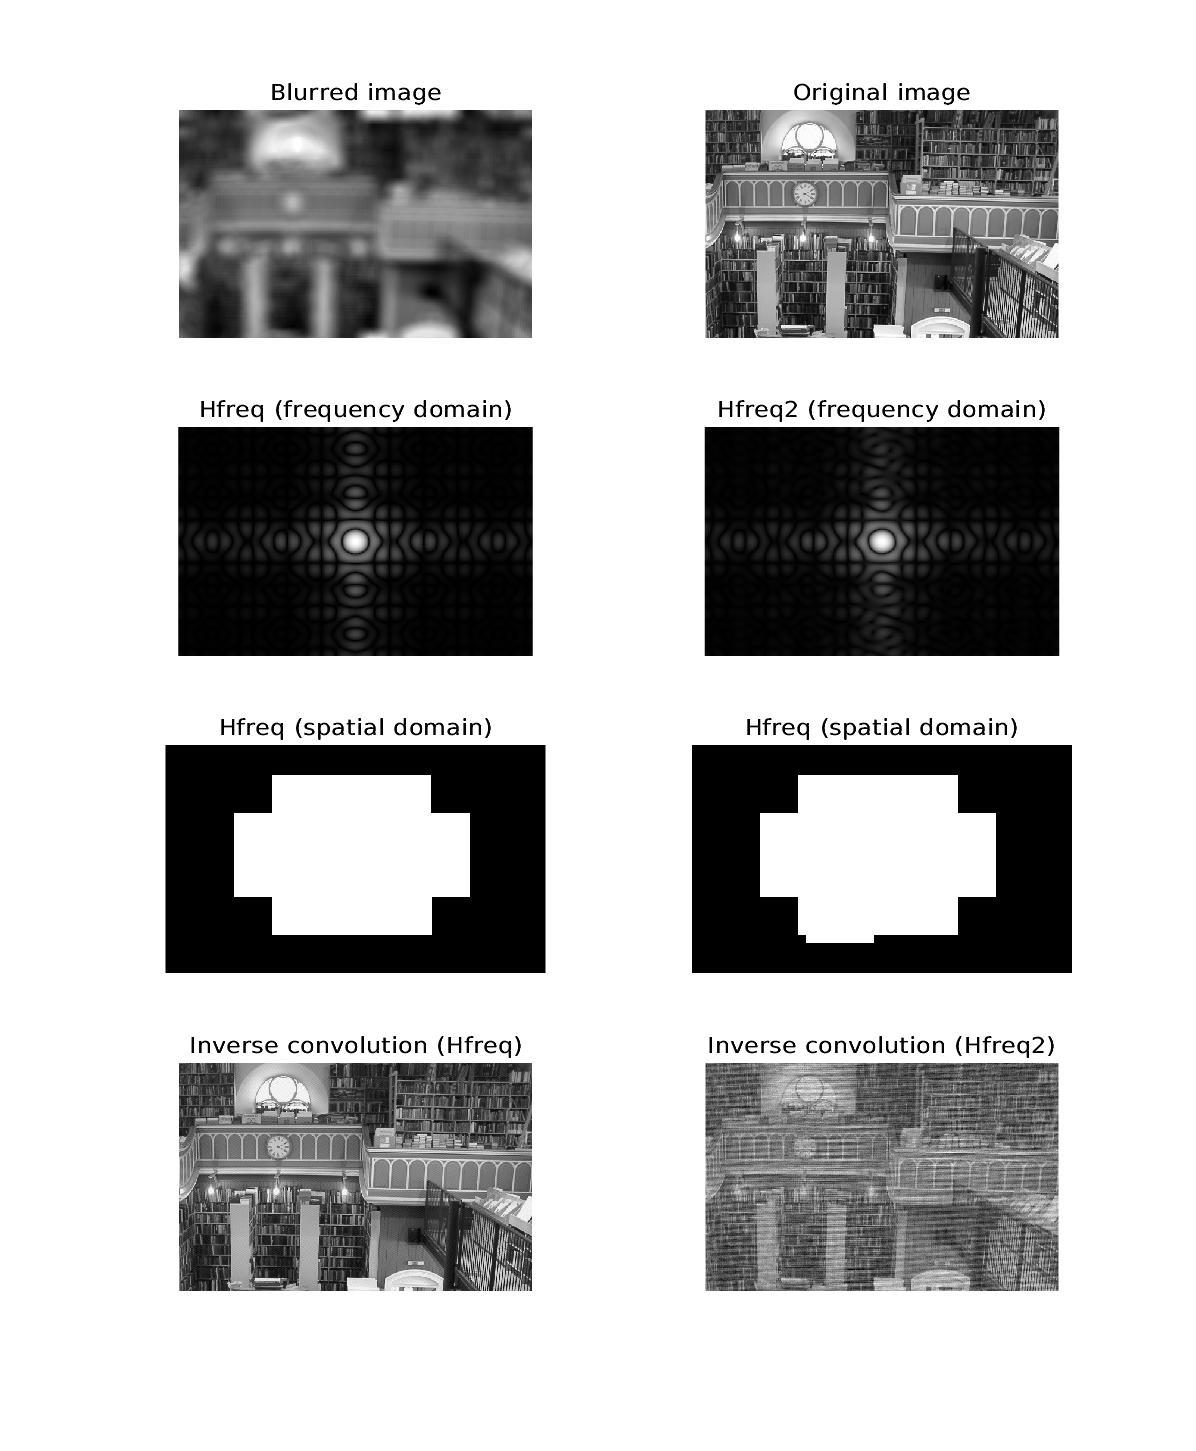
\includegraphics[width=\textwidth]{plot03.jpg}
    \caption{Plots for exercise 3}
    \label{plot03}
\end{figure}

\end{document}